\chapter{MARG Sensors}
\label{ch:MARG}

MARG sensors is a collective term for magnetic, angular rate, and gravitational sensors that encompasses inertial sensors, as well as magnetic field sensors, also referred to as magnetometers. Inertial sensors generally fall into two categories: instruments sensing linear inertial displacement (accelerometers) and rotational inertial rate sensors (gyroscopes). They can be applied in various contexts to quantify vibration, motion, and shock \cite{bhattacharyya_inertial_sensors_applications_13}. Particularly, the development of \gls{MEMS} opened up many medical applications as mentioned in the previous Section \ref{sec:MARG_sensors_medical}. This chapter compiles the functional principles of MARG sensors and introduces \glspl{IMU} as a combination of those. At the end of the chapter the aforementioned GaitWatch device is described in detail.

\section{Accelerometers}

Accelerometers measure the acceleration of an object relative to an inertial frame. Since acceleration cannot be measured directly, the force exerted to a reference mass is obtained and the resultant acceleration is computed according to Newton's second law $\mathbf{F} = m \cdot \mathbf{a}$, where $ \mathbf{F}$ denotes the three-dimensional force vector, $m$ the mass, and $\mathbf{a}$ the three-dimensional acceleration vector. Usually, an accelerometer consists of a small proof mass connected via a spring to the case of the instrument. The proof mass is displaced  by $\Delta x$ with respect to the case, when the instrument experiences a certain acceleration along its sensitive axis. Disregarding drag force, the displacement is directly proportional to the force exerted by the mass and thus to the acceleration. Therefore, by measuring the displacement of the proof mass the acceleration can be obtained. Figure \ref{fig:accelerometer} shows the displacement $\Delta x$ of the mass in respect to the case of the instrument for three different conditions: (a) at rest or in uniform motion, (b) accelerating, and (c) at rest. In cases where the three-dimensional vector of the acceleration is required, three single-axis accelerometers are used. Although a mutually orthogonal mount is common practice, any non-coplanar arrangement is acceptable, as long as the angle between the sensitive axis are known \cite{bhattacharyya_inertial_sensors_applications_13}.


\begin{figure}
\centering
\begin{tikzpicture}[auto, thick, node distance=3cm,>=latex']
    
    \pgftext{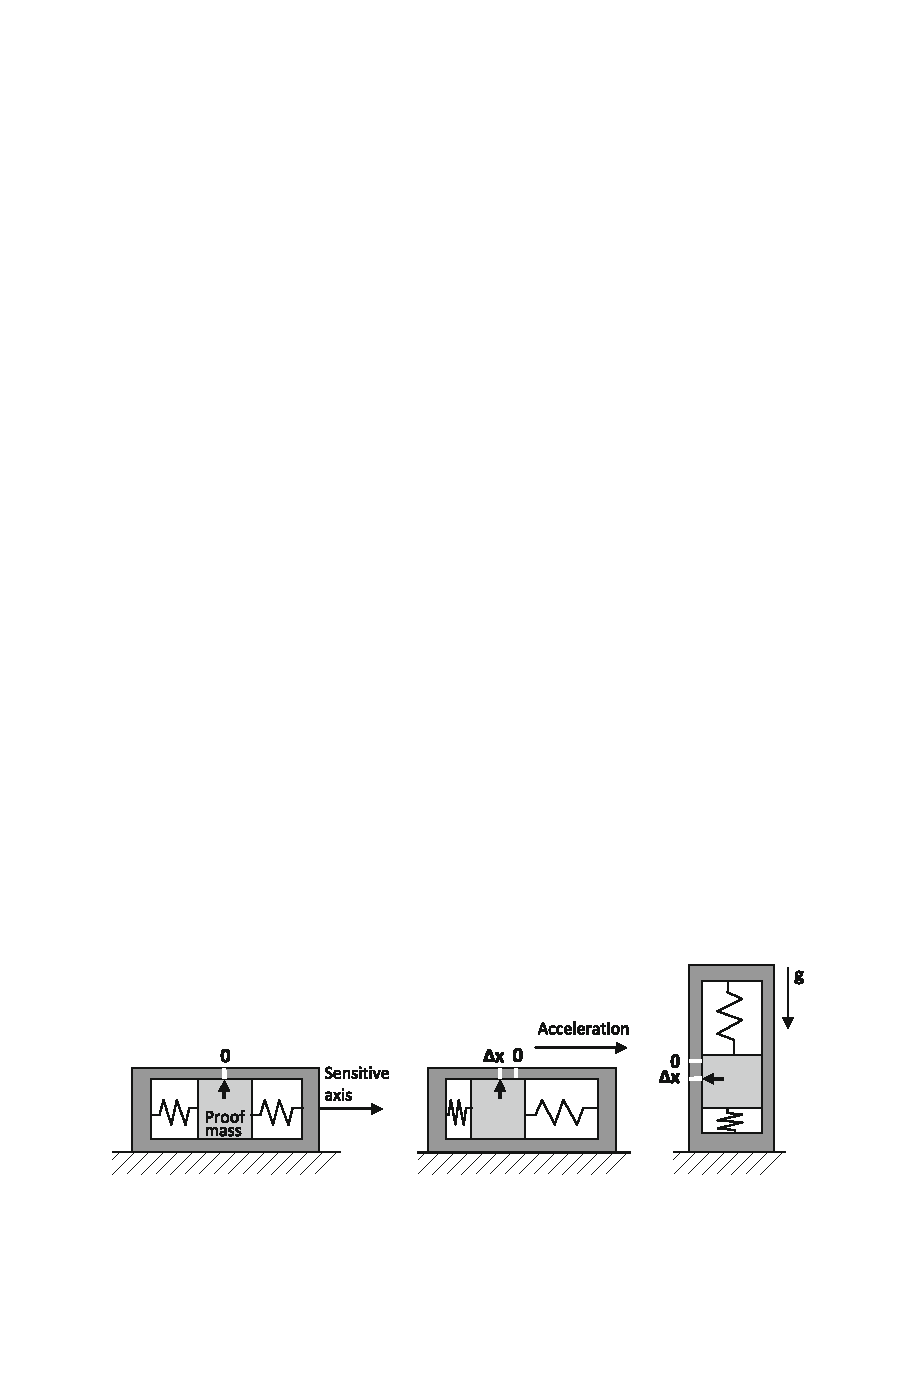
\includegraphics[width=13.5cm]{images/accelerometer}} at (0pt,0pt);
    \node [] (a) at (-6.7, -1.1) {(a)};
    \node [] (b) at (-1.1, -1.1) {(b)};
    \node [] (c) at (3.9, -1.1) {(c)};
    
\end{tikzpicture}
\caption{A mass-and-spring accelerometer under different conditions: (a) at rest or in uniform motion, (b) accelerating, and (c) at rest from \cite{bhattacharyya_inertial_sensors_applications_13}.}
	\label{fig:accelerometer}
\end{figure}

\section{Gyroscopes}

Gyroscopes, also called angular rate sensors, measure angular velocity and are based on the Coriolis Effect. By integrating the angular velocity the rotation angle is obtained \cite{olivares_vicente_signal_2013}.

\section{Magnetometers}

Magnetometers measure the strength and the direction of the magnetic field in a point in space, using the relationship between magnetic fields, movement and induced currents \cite{olivares_vicente_signal_2013}.

\section{Inertial Measurement Units}

Devices using a combination of accelerometers and gyroscopes to measure the orientation of a rigid body with up to six degrees of freedom are referred to as \glspl{IMU}. If they include additional magnetometers they are termed \glspl{MIMU} and can obtain the orientation of the body with up to nine degrees of freedom, whereby the number of degrees of freedom states the number of independent motions, with respect to a reference frame, that are allowed to the body in space.

\glspl{MIMU} are portable and relatively inexpensive. They can be easily attached to the body and thus allow non-clinical longterm application. Their drawbacks are complex calibration procedures and drift behaviour over time, depending on intensity and duration of the measurement interval. Hence, in order to maintain a satisfactory degree of precision, periodical recomputation of the calibration parameters is required \cite{olivares_vicente_signal_2013}.

\subsection{Euler Angles}

Euler angles are one of several ways to describe the rotational orientation of an object and its associated body frame, with respect to the navigation frame, in three-dimensional Euclidean space. They represent a sequence of three elemental rotations about the axis of a coordinate system, defined as follows:

\begin{itemize}

\item The \emph{roll} angle $\phi$ determines the rotation around the $x$-axis
\item The \emph{pitch} angle $\theta$ determines the rotation around the $y$-axis
\item The \emph{yaw} angle $\psi$ determines the rotation around the $z$-axis

\end{itemize}


\begin{figure}
\centering

%Angle Definitions
%-----------------

%set the plot display orientation
%synatax: \tdplotsetdisplay{\theta_d}{\phi_d}
\tdplotsetmaincoords{60}{110}

%define polar coordinates for some vector
\pgfmathsetmacro{\rvec}{.8}
\pgfmathsetmacro{\thetavec}{30}
\pgfmathsetmacro{\phivec}{60}

%start tikz picture, and use the tdplot_main_coords style to implement the display 
%coordinate transformation provided by 3dplot
\begin{tikzpicture}[scale=6,tdplot_main_coords]

%set up some coordinates 
%-----------------------
\coordinate (O) at (0,0,0);

%determine a coordinate (P) using (r,\theta,\phi) coordinates.  This command
%also determines (Pxy), (Pxz), and (Pyz): the xy-, xz-, and yz-projections
%of the point (P).
%syntax: \tdplotsetcoord{Coordinate name without parentheses}{r}{\theta}{\phi}
\tdplotsetcoord{P}{\rvec}{\thetavec}{\phivec}

%draw figure contents
%--------------------

%draw the main coordinate system axes
\draw[thick,->] (0,0,0) -- (1,0,0) node[anchor=north east]{$x$};
\draw[thick,->] (0,0,0) -- (0,1,0) node[anchor=north west]{$y$};
\draw[thick,->] (0,0,0) -- (0,0,1) node[anchor=south]{$z$};

%draw a vector from origin to point (P) 
\draw[-stealth,color=red] (O) -- (P);

%draw projection on xy plane, and a connecting line
\draw[dashed, color=red] (O) -- (Pxy);
\draw[dashed, color=red] (P) -- (Pxy);

%draw the angle \phi, and label it
%syntax: \tdplotdrawarc[coordinate frame, draw options]{center point}{r}{angle}{label options}{label}
\tdplotdrawarc{(O)}{0.2}{0}{\phivec}{anchor=north}{$\phi$}


%set the rotated coordinate system so the x'-y' plane lies within the
%"theta plane" of the main coordinate system
%syntax: \tdplotsetthetaplanecoords{\phi}
\tdplotsetthetaplanecoords{\phivec}

%draw theta arc and label, using rotated coordinate system
\tdplotdrawarc[tdplot_rotated_coords]{(0,0,0)}{0.5}{0}{\thetavec}{anchor=south west}{$\theta$}

%draw some dashed arcs, demonstrating direct arc drawing
\draw[dashed,tdplot_rotated_coords] (\rvec,0,0) arc (0:90:\rvec);
\draw[dashed] (\rvec,0,0) arc (0:90:\rvec);

%set the rotated coordinate definition within display using a translation
%coordinate and Euler angles in the "z(\alpha)y(\beta)z(\gamma)" euler rotation convention
%syntax: \tdplotsetrotatedcoords{\alpha}{\beta}{\gamma}
\tdplotsetrotatedcoords{\phivec}{\thetavec}{0}

%translate the rotated coordinate system
%syntax: \tdplotsetrotatedcoordsorigin{point}
\tdplotsetrotatedcoordsorigin{(P)}

%use the tdplot_rotated_coords style to work in the rotated, translated coordinate frame
\draw[thick,tdplot_rotated_coords,->] (0,0,0) -- (.5,0,0) node[anchor=north west]{$x'$};
\draw[thick,tdplot_rotated_coords,->] (0,0,0) -- (0,.5,0) node[anchor=west]{$y'$};
\draw[thick,tdplot_rotated_coords,->] (0,0,0) -- (0,0,.5) node[anchor=south]{$z'$};

%WARNING:  coordinates defined by the \coordinate command (eg. (O), (P), etc.)
%cannot be used in rotated coordinate frames.  Use only literal coordinates.  

%draw some vector, and its projection, in the rotated coordinate frame
\draw[-stealth,color=blue,tdplot_rotated_coords] (0,0,0) -- (.2,.2,.2);
\draw[dashed,color=blue,tdplot_rotated_coords] (0,0,0) -- (.2,.2,0);
\draw[dashed,color=blue,tdplot_rotated_coords] (.2,.2,0) -- (.2,.2,.2);

%show its phi arc and label
\tdplotdrawarc[tdplot_rotated_coords,color=blue]{(0,0,0)}{0.2}{0}{45}{anchor=north west,color=black}{$\phi'$}

%change the rotated coordinate frame so that it lies in its theta plane.
%Note that this overwrites the original rotated coordinate frame
%syntax: \tdplotsetrotatedthetaplanecoords{\phi'}
\tdplotsetrotatedthetaplanecoords{45}

%draw theta arc and label
\tdplotdrawarc[tdplot_rotated_coords,color=blue]{(0,0,0)}{0.2}{0}{55}{anchor=south west,color=black}{$\theta'$}

\end{tikzpicture}

\caption{Euler angles from \cite{olivares_vicente_gaitwatch_2013}.}
	\label{fig:GaitWatch_placement}
\end{figure}


\begin{figure}
\centering

\begin{subfigure}[]{0.45\textwidth}
      \caption{Initial situation}

%set the plot display orientation
\tdplotsetmaincoords{60}{110}

\begin{tikzpicture}[scale=3.5,tdplot_main_coords]

%draw the main coordinate system axes
\draw[thick,->] (0,0,0) -- (1,0,0) node[anchor=north east]{$x$};
\draw[thick,->] (0,0,0) -- (0,1,0) node[anchor=north west]{$y$};
\draw[thick,->] (0,0,0) -- (0,0,1) node[anchor=south]{$z$};

\draw[thick,red,->] (0,0,0) -- (.7,0,0) node[anchor=north west]{$x_0$};
\draw[thick,red,->] (0,0,0) -- (0,.7,0) node[anchor=north west]{$y_0$};
\draw[thick,red,->] (0,0,0) -- (0,0,.7) node[anchor=north west]{$z_0$};

\end{tikzpicture}
\end{subfigure}
\quad
\begin{subfigure}[]{0.45\textwidth}
                \caption{Rotation by $\psi$ around $z$}

%set the plot display orientation
%syntax: \tdplotsetdisplay{\theta_d}{\phi_d}
\tdplotsetmaincoords{60}{110}

%define polar coordinates for some vector
\pgfmathsetmacro{\phivec}{0}
\pgfmathsetmacro{\thetavec}{0}
\pgfmathsetmacro{\psivec}{25}

\begin{tikzpicture}[scale=3.5,tdplot_main_coords]

%draw the main coordinate system axes
\draw[thick,->] (0,0,0) -- (1,0,0) node[anchor=north east]{$x$};
\draw[thick,->] (0,0,0) -- (0,1,0) node[anchor=north west]{$y$};
\draw[thick,->] (0,0,0) -- (0,0,1) node[anchor=south]{$z$};

\draw[thick,red,->] (0,0,0) -- (.7,0,0) node[anchor=north west]{$x_0$};
\draw[thick,red,->] (0,0,0) -- (0,.7,0) node[anchor=north west]{$y_0$};

\tdplotsetrotatedcoords{0}{0}{25}

%use the tdplot_rotated_coords style to work in the rotated, translated coordinate frame
\draw[thick,blue,tdplot_rotated_coords,->] (0,0,0) -- (.7,0,0) node[anchor=north west]{$x_1$};
\draw[thick,blue,tdplot_rotated_coords,->] (0,0,0) -- (0,.7,0) node[anchor=west]{$y_1$};
\draw[thick,blue,tdplot_rotated_coords,->] (0,0,0) -- (0,0,.7) node[anchor=north west]{$z_1=z_0$};

%show its psi arc and label
%syntax: \tdplotdrawarc[coordinate frame, draw options]{center point}{r}{angle}{label options}{label}
\tdplotdrawarc[-stealth]{(0,0,0)}{0.35}{0}{\psivec}{anchor=north}{$\psi$}

%draw dashed arcs
\draw[dashed] (0.7,0,0) arc (0:115:0.7);

\end{tikzpicture}
\end{subfigure}

\begin{subfigure}[]{0.45\textwidth}
                \caption{Rotation by $\theta$ around $y_1$ }

\tdplotsetmaincoords{60}{170}

\begin{tikzpicture}[scale=3.5,tdplot_main_coords]

%draw the main coordinate system axes
\draw[thick,->] (0,0,0) -- (1,0,0) node[anchor=north east]{$x$};
\draw[thick,->] (0,0,0) -- (0,1,0) node[anchor=north west]{$y$};
\draw[thick,->] (0,0,0) -- (0,0,1) node[anchor=south]{$z$};

\tdplotsetrotatedcoords{0}{0}{25}

\draw[thick,red,tdplot_rotated_coords,->] (0,0,0) -- (.7,0,0) node[anchor=north west]{$x_1$};
\draw[thick,red,tdplot_rotated_coords,->] (0,0,0) -- (0,0,.7) node[anchor=north west]{$z_1$};

\tdplotsetmaincoords{60}{145}
\tdplotsetrotatedcoords{0}{25}{0}

\draw[thick,tdplot_rotated_coords,blue,->] (0,0,0) -- (.7,0,0) node[anchor=north west]{$x_2$};
\draw[thick,tdplot_rotated_coords,blue,->] (0,0,0) -- (0,.7,0) node[anchor=west]{$y_2=y_1$};
\draw[thick,tdplot_rotated_coords,blue,->] (0,0,0) -- (0,0,.7) node[anchor=north east]{$z_2$};

\tdplotsetthetaplanecoords{0}
\draw[dashed,tdplot_rotated_coords] (0.7,0,0) arc (0:115:0.7);
\tdplotdrawarc[-stealth,tdplot_rotated_coords]{(0,0,0)}{0.55}{0}{25}{anchor=north}{$\theta$}

\end{tikzpicture}
\end{subfigure}
\quad
\begin{subfigure}[]{0.45\textwidth}
    \caption{Rotation by $\phi$ around $x_2$}

\tdplotsetmaincoords{60}{130}

\begin{tikzpicture}[scale=3.5,tdplot_main_coords]

%draw the main coordinate system axes
\draw[thick,->] (0,0,0) -- (1,0,0) node[anchor=north east]{$x$};
\draw[thick,->] (0,0,0) -- (0,1,0) node[anchor=north west]{$y$};
\draw[thick,->] (0,0,0) -- (0,0,1) node[anchor=south]{$z$};

\tdplotsetmaincoords{60}{105}
\tdplotsetrotatedcoords{0}{25}{0}

\draw[thick,tdplot_rotated_coords,blue,->] (0,0,0) -- (.7,0,0) node[anchor=north west]{$x_3=x_2$};
\draw[thick,tdplot_rotated_coords,red,->] (0,0,0) -- (0,.7,0) node[anchor=west]{$y_2$};
\draw[thick,tdplot_rotated_coords,red,->] (0,0,0) -- (0,0,.7) node[anchor=north east]{$z_2$};

\tdplotsetrotatedthetaplanecoords{90}
\draw[dashed,tdplot_rotated_coords] (0.7,0,0) arc (0:90:0.7);

\draw[dashed,tdplot_rotated_coords] (0.7,0,0) arc (0:-23:0.7);

\tdplotsetmaincoords{60}{125}
\tdplotsetrotatedcoords{10}{40}{20}

\draw[thick,tdplot_rotated_coords,blue,->] (0,0,0) -- (0,.63,0) node[anchor=west]{$y_3$};
\draw[thick,tdplot_rotated_coords,blue,->] (0,0,0) -- (0,0,1.1) node[anchor=north east]{$z_3$};

\end{tikzpicture}
\end{subfigure}


\caption{Euler angles from \cite{olivares_vicente_gaitwatch_2013}.}
	\label{fig:GaitWatch_placement}
\end{figure}




\section{The GaitWatch}

The above mentioned GaitWatch device we used to gather the movement data was designed to monitor the motion of patients while attached to the body. It was developed at the Department of Neurology of the Ludwig-Maximilians University in Munich, Germany, in association with the Department of Signal Theory, Telematics and Communications of the University of Granada, Spain. The system is composed of a set of embedded magnetic and inertial sensors wired to a box containing a microcontroller. This microcontroller is in charge of collecting data from the embedded box sensors, as well as from the external measurement units, and storing them on a memory card. The various units are placed at the patient's trunk, arms, thighs, and shanks as shown in Figure \ref{fig:GaitWatch_placement}. The components of the three different kinds of subunits are described below:


\begin{itemize}

\item \textsc{Type A} -- thighs and shanks: 

IMU Analog Combo Board with 5 Degrees of Freedom \cite{IMU5}, containing an IDG500 biaxial gyroscope, from which only y-axis is actually used, with a measurement range of ±500\,°/s \cite{IDG500} and a ±3\,g triaxial accelerometer, ADXL335 \cite{ADXL335}.

\item \textsc{Type B} -- arms:

IDG500 biaxial gyroscope with a measurement range of ±500\,°/s \cite{IDG500}.

\item \textsc{Type C} -- trunk:

ADXL345 triaxial accelerometer with a programmable measurement range of ±2/±4/±8/±16\,g \cite{ADXL345},
IMU3000 triaxial gyroscope with a programmable measurement range of ±250/±500/±1000/±3000°/s \cite{IMU3000}, 
Micromag3 \allowbreak triaxial magnetometer with a measurement range of ±11\,Gauss \cite{MicroMag3}, AL-XAVRB board containing an AVR ATxmega processor \cite{AVRATxmega}.

\end{itemize}

\begin{figure}
	\centering
	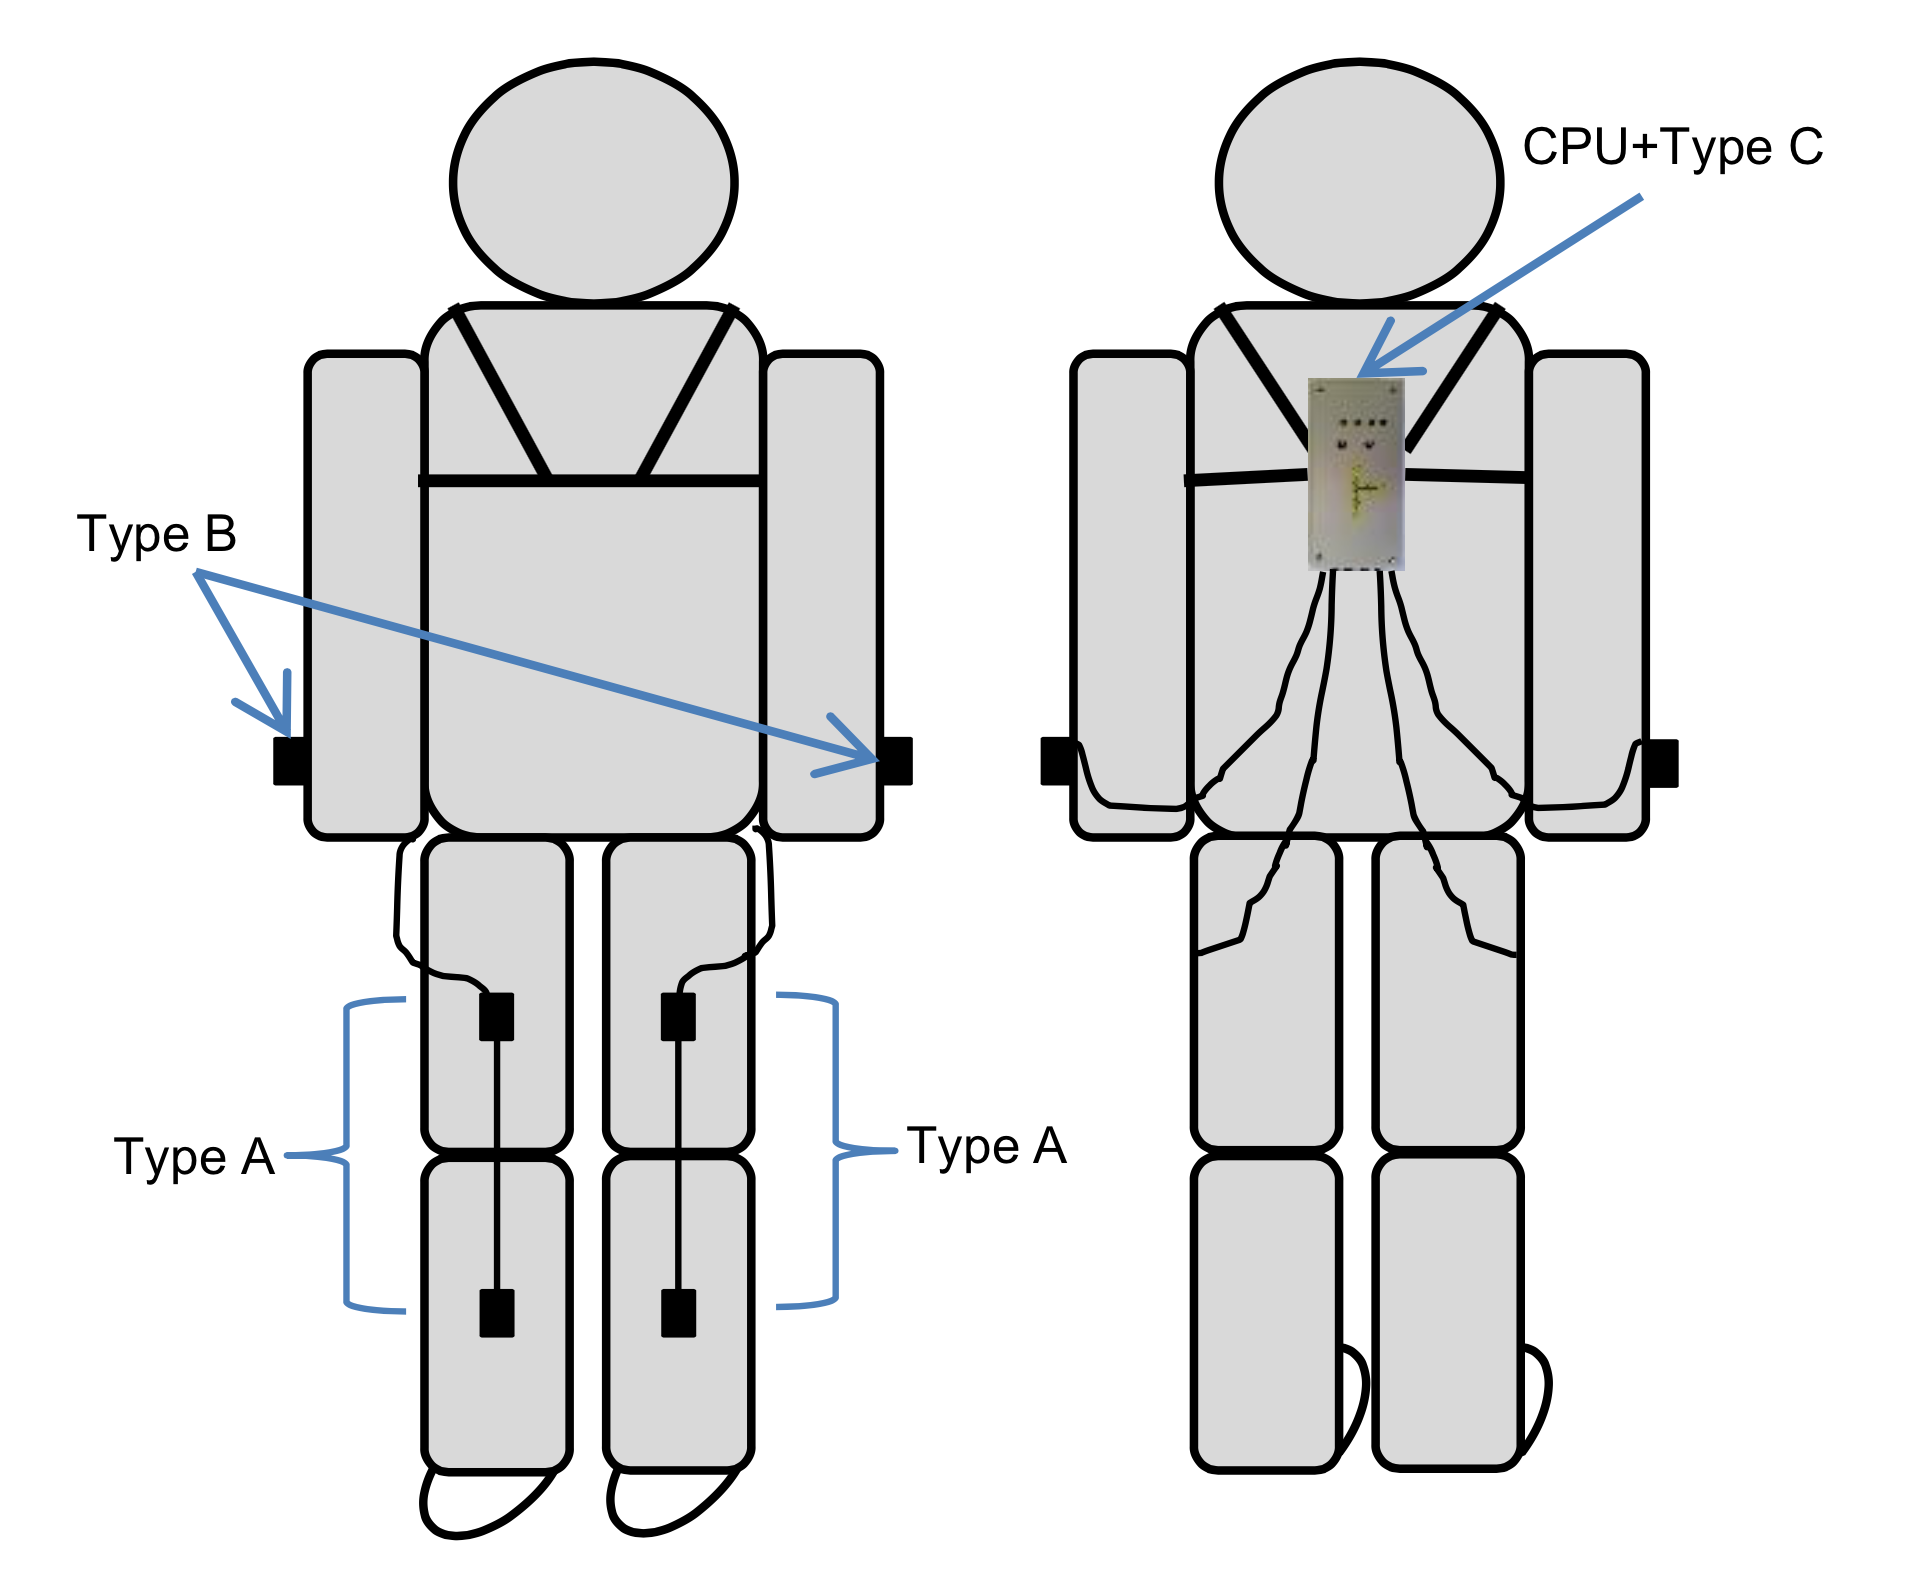
\epsfig{file=images/GaitWatch_placement, width=9cm}
	\caption{Placement of the GaitWatch components at the body from \cite{olivares_vicente_gaitwatch_2013}.}
	\label{fig:GaitWatch_placement}
\end{figure}
